\subsection{Hierarchical Clustering}

Hierarchical cluster is defined by a stepwise algorithm which merges two objects at each step,the two which have the least dissimilarity.

  
Accroding to the clusters we did in GMM, we find out that a few data constitute a big cluster with low purity while other clusters are more centralized with high purity. It turns out that most of the datas should be classified into one cluster.

In this case, the group choose standardized euclidean and minimim dissimilarity (single linkage) to draw the dendrogram, which is shown in fig.3. The branches of this tree are cut at a level where the jump in levels of two consecutive nodes is large. From our dendrogram, we can cut it into 3 classes.
%kommentar
\begin{figure}[!ht]
	\centering
	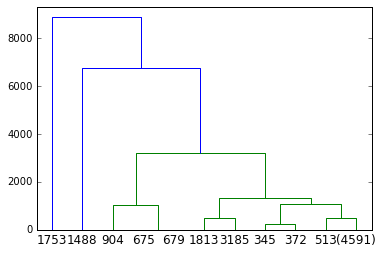
\includegraphics[width=0.7\textwidth]{Fig/HC1.png}
	\vspace{-5pt}
	\caption{The dendrogram drawn by single linkage cluster analyses of the standardized euclidean distence}
	\label{fig:HC1}
\end{figure}




